%!TEX spellcheck
%!TEX root = ../bachelor_paper.tex
\documentclass[../bachelor_paper.tex]{subfiles}
\graphicspath{{\subfix{images/}}}
\begin{document}

\chapter{Platform}
    \label{ch:plat}

\section{Instruction Set Architecture}
We chose the open RISC-V \ac{ISA} as our target. RISC-V is a free to use \acf{ISA} which originates from work conducted at Berkley University \cite{HistoryRISCV2022}. This royalty-free aspect has lead to frequent use in academic papers and emergence of numerous open and closed source hardware designs using the \ac{ISA}. The architecture is a basic RISC-like load/store architecture featuring an unprivileged and privileged specification \cite{RISCVInstructionSet2022}. The Pulp Platform, which this thesis is based on uses unprivileged RISC-V and is published under the SolderPad Hardware License v0.51 \cite{GitHubPulpplatformPulpissimo2021}.

\section{Base IP}
    \label{sec:plat:base}
We base our design on the Pulpissimo microcontroller IP provided by the ETH Z\"urich and University of Bologna \cite{schiavoneQuentinUltraLowPowerPULPissimo2018}. The core used in the design is the CV32E40P, formerly known and here (for simplicity) referred to as RI5CY \cite{gautschiNearThresholdRISCVCore2017}. RI5CY is a 32-bit core with a single-issue, in-order, 4-stage pipeline implementing the RV32IM[F]C instruction set. Floating point support can be enabled and disabled ([F]) depending on requirements towards the core. We will have floating point support enabled as dedicated hardware \acp{FPU} have become rather common even in embedded \acp{SoC}. RI5CY does support several nonstandard extensions to the RISC-V \ac{ISA} such has \acl{HWL}, dot product multiplication (also referred to as multiply-accumulate), nonstandard floating point formats, as well as packed SIMD operations.

\subsection{Pipeline}
    \label{sec:plat/pipe}
As seen in Figure \ref{fig:plat/base/blockdia}, RI5CY consists of 4 pipeline stages. Stage one is an instruction fetch stage using a 4 entry prefetch buffer as well as a \ac{HWL} controller, which we will go into detail about in Section \ref{sub:plat/ip/ctrl}. Stage 2 is the instruction decode stage, containing the RISC-V decoder as well as the register file and \ac{HWL} registers. Stage 3 is the execute stage featuring an \ac{ALU} for arithmetic and logic operations except multiplication, as well as a multi-cycle multiplication unit which can also perform multiply accumulate operations. Additionally, if enabled, the exec stage also contains the \ac{FPU} which we will go further into in Section \ref{sub:plat/ip/fpu}. The 4th and final pipeline stage contains the load/store unit as well as the register write-back. The main design goal of the RI5CY core was to provide a low power, high performance \ac{DSP}-focused core \cite{gautschiNearThresholdRISCVCore2017}, which is reflected in the chosen set of optimizations.

\begin{figure}
    \centering
    %\includesvg[width=0.6\columnwidth]{ri5cy_blockdiagram}
    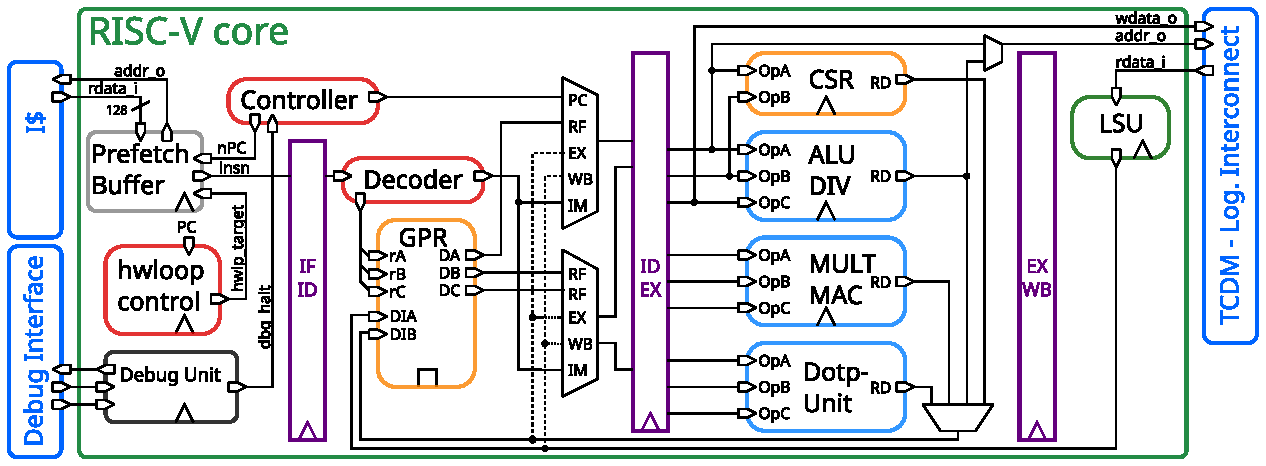
\includegraphics[width=\textwidth]{img/ri5cy_blockdiagram.pdf}
    \caption{Block diagram of the RI5CY pipeline}
    \label{fig:plat/base/blockdia}
\end{figure}

\subsection{Instruction memory architecture}
RI5CY does not feature a full level 1 cache. Instead it contains a 4-instruction deep prefetch buffer inside the instruction fetch stage. This buffer is able to preload up to 4 instructions for execution and is used as a minimalist loop buffer for the \ac{HWL} implementation described in Section \ref{sub:plat/ip/ctrl}.

\subsection{Control flow}
    \label{sub:plat/ip/ctrl}
RI5CY implements a simple \emph{branch-not-taken} prediction strategy. However, in order to reduce branching overhead, RI5CY implements a \acl{HWL} (also called zero-overhead-loops) extension to the RISC-V \ac{ISA}. \\
The \texttt{lp.setup} instructions allow for set-up of a hardware loop within a single step, additional instructions \texttt{lp.start}, \texttt{lp.end}, \texttt{lp.count}, and \texttt{lp.counti} allow for explicit write access to the individual registers used for hardware looping. Subsequent loop iterations are handled by the instruction fetch stage and thus cause no stalls in the pipeline as long as loop instructions fit inside the prefetch buffer. A \ac{HWL}-based jump is executed when the difference between the program counter and the loop end point stored in the \ac{HWL} registers is zero, as long as the loop counter has not reached zero. When the counter reaches zero, normal execution is resumed. The \ac{HWL} controller in RI5CY is configured to support 2 levels of nested loops, as diminishing speedup to area increase was observed at higher levels \cite{gautschiNearThresholdRISCVCore2017}.

Apart from \ac{DSP} calculations, the inclusion of \acp{HWL} has also shown to provide significant speedups for other loop heavy calculations. Experiments by Vre\v{c}a et al.\ \cite{vrecaAcceleratingDeepLearning2020} have shown that the inclusion of \acp{HWL} alone have provided a 29\% reduction in clock cycle count compared to a baseline with no optimizations (loop unrolling, \acp{HWL}, dot product).

\subsection{Floating point support}
    \label{sub:plat/ip/fpu}
The \ac{FPU} is enabled for the experiments in this thesis. RI5CY uses FPnew, a highly configurable open-source multiformat floating point unit \cite{machFPnewOpenSourceMultiformat2021}. FPnew is split into four different data paths, each of them having configurable datapath depth and width, and supports transprecision computing \cite{malossiTransprecisionComputingParadigm2018}. In addition to 32 bit single precision (FP32), and 64 bit double precision (FP64) it supports half-precision (FP16), 16 bit bfloats (FP16alt), as well as an 8 bit custom format (FP8). For RI5CY, only support for FP32, FP16, and FP16alt is enabled. The four data paths implement the functions \ac{ADDMUL}, \ac{DIVSQRT}, \ac{COMP}, and \ac{CONV} respectively. These datapaths can be either generated in parallel to support one data format per lane or merged to be multiformat. They can also be disabled completely, if required. For RI5CY, \ac{ADDMUL} and \ac{COMP} are enabled in merged mode to save power and area allowing one FP32 operation or a packed vector of either 2 FP16 or FP16alt, \ac{COMP} is implemented in parallel mode allowing for one FP32 operation or a packed vector of either 2 FP16 or FP16alt, and \ac{DIVSQRT} is disabled outright (as seen in Table \ref{tab:plat/base/fpu}). All pipelines have a depth of 1 as clock requirements are relatively relaxed for smaller \acp{MCU} like RI5CY, so floating point operations can complete within a single cycle. The \ac{FPU} is integrated into the \ac{APU} port of the execution stage. These details are important for Chapter \ref{ch:arch}, as this configuration means all FPU operations on RI5CY complete within a single cycle and thus only the percentage of FPU instructions has to be measured.

The \ac{FPU} is integrated into RI5CY using the cores \acl{APU} interface.

\begin{table}
    \centering
    \caption{Configuration of the FPU for RI5CY \cite{machFPnewOpenSourceMultiformat2021}}
    \begin{tabular}{lllll}
        \hline \\[-0.9em]
        \textbf{Format} & \multicolumn{4}{l}{\textbf{Implementation} (number of cycles, number of lanes)}   \\
                        & \ac{ADDMUL}   & \ac{DIVSQRT}  & \ac{COMP}     & \ac{CONV}     \\
        \hline \\[-0.9em]
        FP32            & merged (1,1)  & disabled (-,-)& parallel (1,1)& merged (1,2)  \\
        FP16            & merged (1,2)  & disabled (-,-)& parallel (1,2)& merged (1,2)  \\
        FP16alt         & merged (1,2)  & disabled (-,-)& parallel (1,2)& merged (1,2)  \\
        \hline
    \end{tabular}
    \label{tab:plat/base/fpu}
\end{table}

\section{Xilinx ZYNQ-7000 SoC}
The hardware used is a ZedBoard by Digilent. It is equipped with a Zynq-7000 All Programmable \ac{SoC} by Xilinx and natively supported by Pulpissimo. The Zynq-7000 processor features a \ac{PL} as well as a Dual ARM Cortex-A9 MPCore hard IP able to run Linux. The hard IP and \ac{PL} are connected via an AXI bus which can be configured using block diagrams inside the Vivado design environment \cite{Zynq7000SoC}. An architectural block diagram can be seen in Figure \ref{fig:arch/comm/zynq}.


% Render bibliograhy and acronyms if rendered standalone
\isstandalone
\bibliographystyle{IEEEtran}
\bibliography{bibliography}
\subfile{abbreviations.tex}
\fi

\end{document} 
